\documentclass[12pt,letterpaper]{article}
\usepackage[utf8]{inputenc}
\usepackage[spanish]{babel}
\usepackage{graphicx}
\usepackage[left=2cm,right=2cm,top=2cm,bottom=2cm]{geometry}
\usepackage{graphicx}
\usepackage{float}
\usepackage{amsmath}
\usepackage{stackrel} 
\usepackage{multirow}
\usepackage{enumerate}
\renewcommand{\labelitemi}{$-$}
\renewcommand{\labelitemii}{$\cdot$}

\begin{document}

\title{Caratula}

\begin{titlepage}
\begin{center}
\large{UNIVERSIDAD PRIVADA DE TACNA}\\
\vspace*{-0.025in}
\begin{figure}[htb]
\begin{center}

\includegraphics[width=7cm]{./images/logo}
\end{center}
\end{figure}
\vspace*{0.15in}
INGENIERIA DE SISTEMAS  \\

\vspace*{0.3in}
\begin{large}
\textbf{TITULO:} \\
\end{large}

\vspace*{0.1in}
\begin{Large}
\textbf{Informe de Laboratorio 02: Modelando Datos en Power BI} \\

\end{Large}

\vspace*{0.3in}
\begin{Large}
\textbf{CURSO:} \\
\end{Large}

\vspace*{0.1in}
\begin{large}
INTELIGENCIA DE NEGOCIOS\\
\end{large}

\vspace*{0.3in}
\begin{Large}
\textbf{DOCENTE:} \\
\end{Large}

\vspace*{0.1in}
\begin{large}
 Ing. Patrick Cuadros Quiroga\\
\end{large}

\vspace*{0.4in}
\vspace*{0.1in}
\begin{large}
\textbf{INTEGRANTES:} \\
\begin{flushleft}
Apaza Mamani, Edward Hernàn \hfill	(2018060915)\\

\centering  %CENTRA UN TEXTO
\vspace*{0.9in}
\begin{large}
Tacna\\ 22-08-2019
\end{large}

\end{flushleft}
\end{large}
\end{center}

\end{titlepage}


\tableofcontents % INDICE
\thispagestyle{empty} % INDICE SIN NUMERO
\newpage
\setcounter{page}{1} % REINICIAR CONTADOR DE PAGINAS DESPUES DEL INDICE


\section{Ejercicio 1: Conectando a Power BI a datos} 
\subsection{Tarea 1: Conectar a datos existentes}
\begin{center}
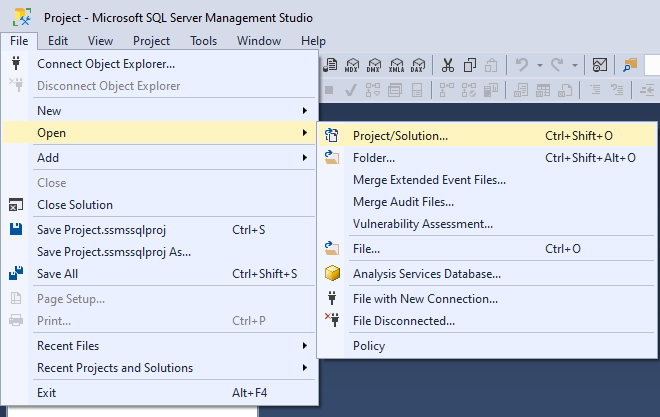
\includegraphics[width=10cm]{images/1}\newline
\end{center}
\begin{center}
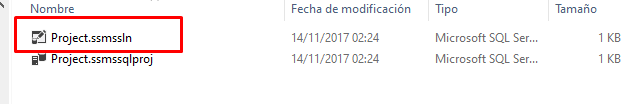
\includegraphics[width=10cm]{images/2}\newline
\end{center}
\begin{center}
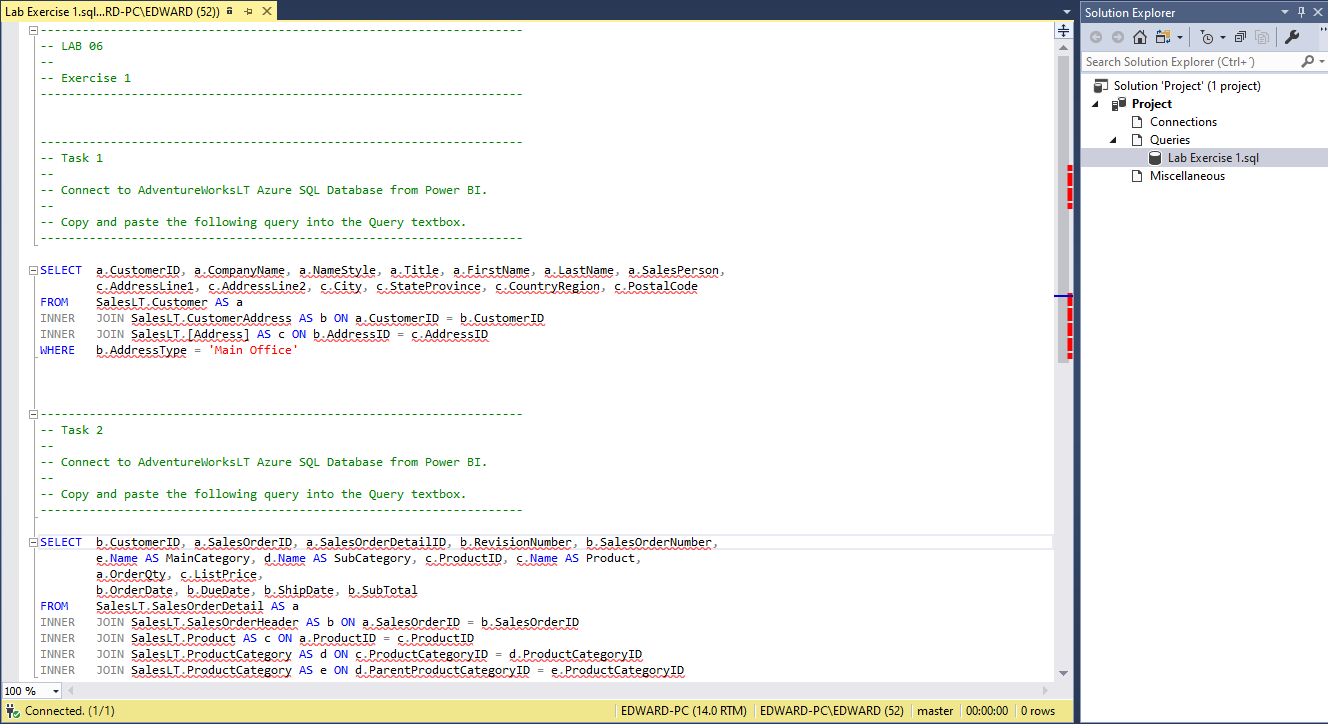
\includegraphics[width=15cm]{images/3}\newline
\end{center}
\begin{center}
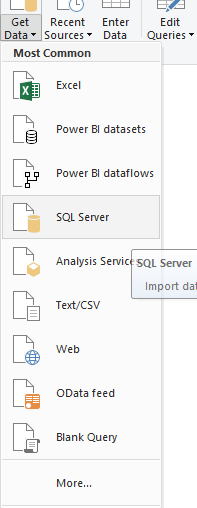
\includegraphics[width=3cm]{images/4}\newline
\end{center}
\begin{center}
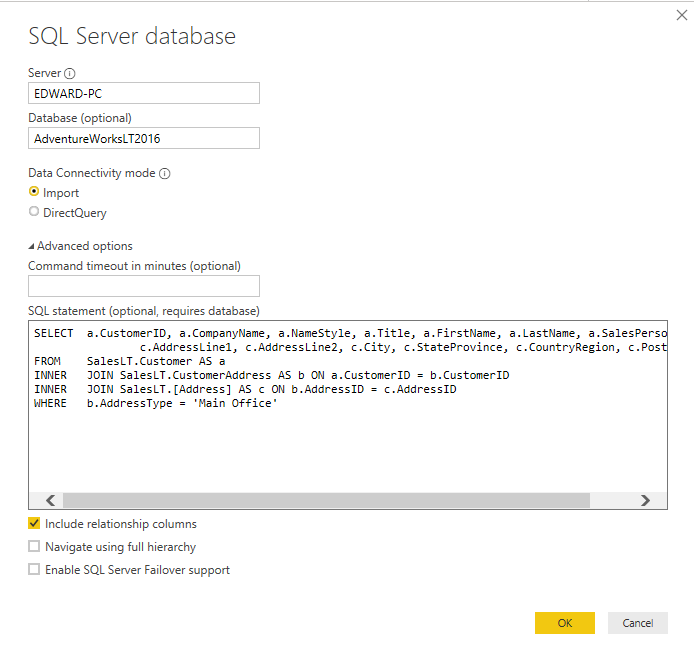
\includegraphics[width=15cm]{images/5}\newline
\end{center}
\begin{center}
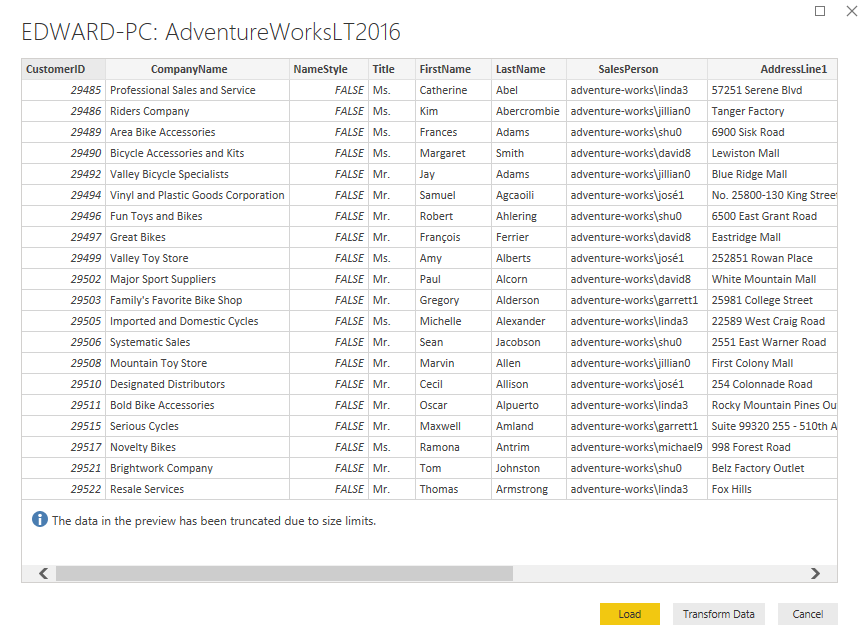
\includegraphics[width=15cm]{images/6}\newline
\end{center}
\begin{center}
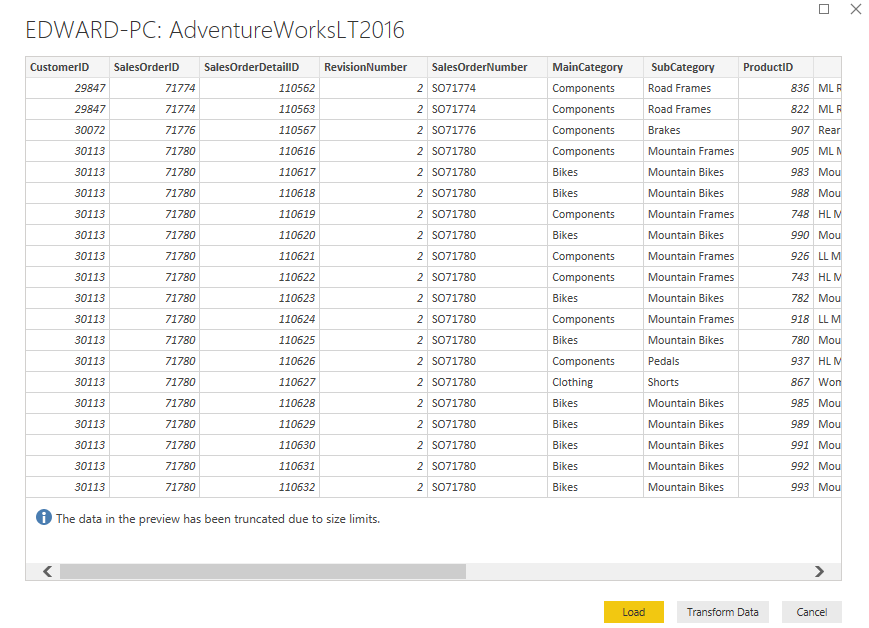
\includegraphics[width=15cm]{images/7}\newline
\end{center}
\subsection{Tarea 2: Graficar Datos}
\begin{center}
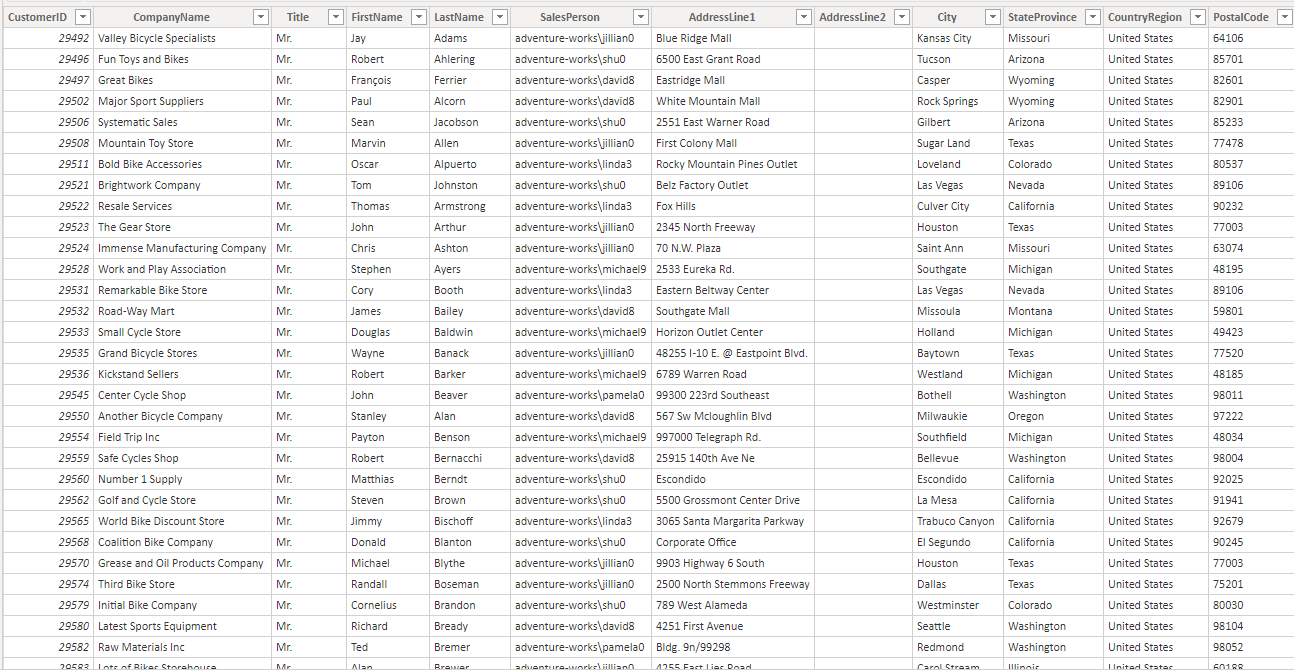
\includegraphics[width=15cm]{images/11}\newline
\end{center}
\begin{center}
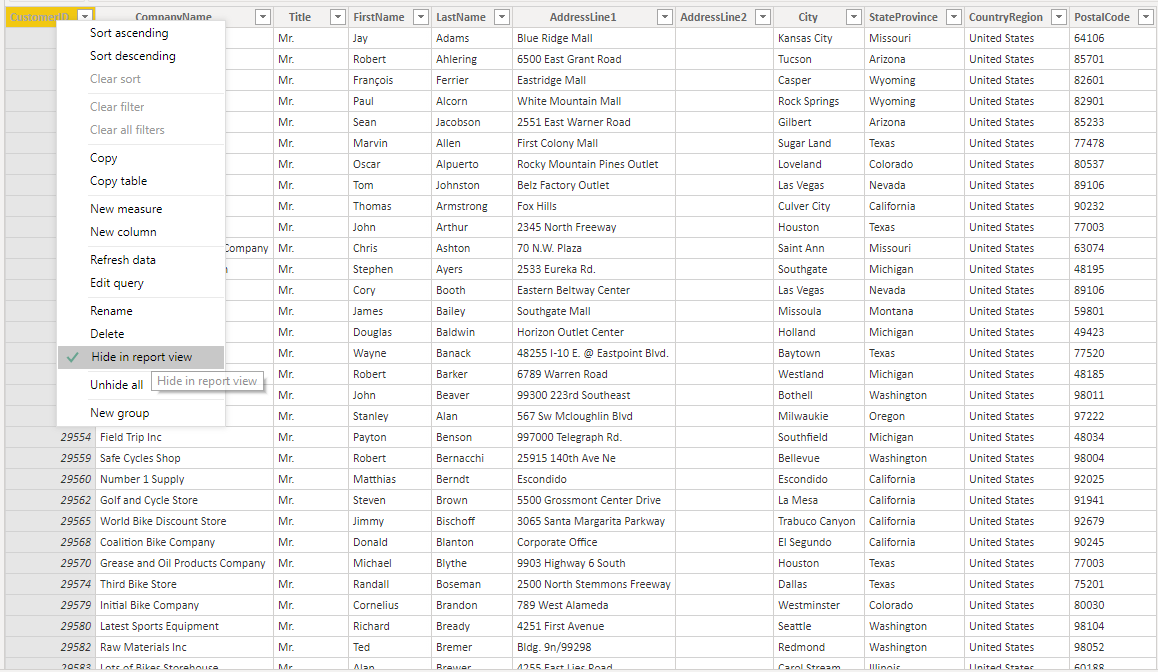
\includegraphics[width=15cm]{images/22}\newline
\end{center}
\begin{center}
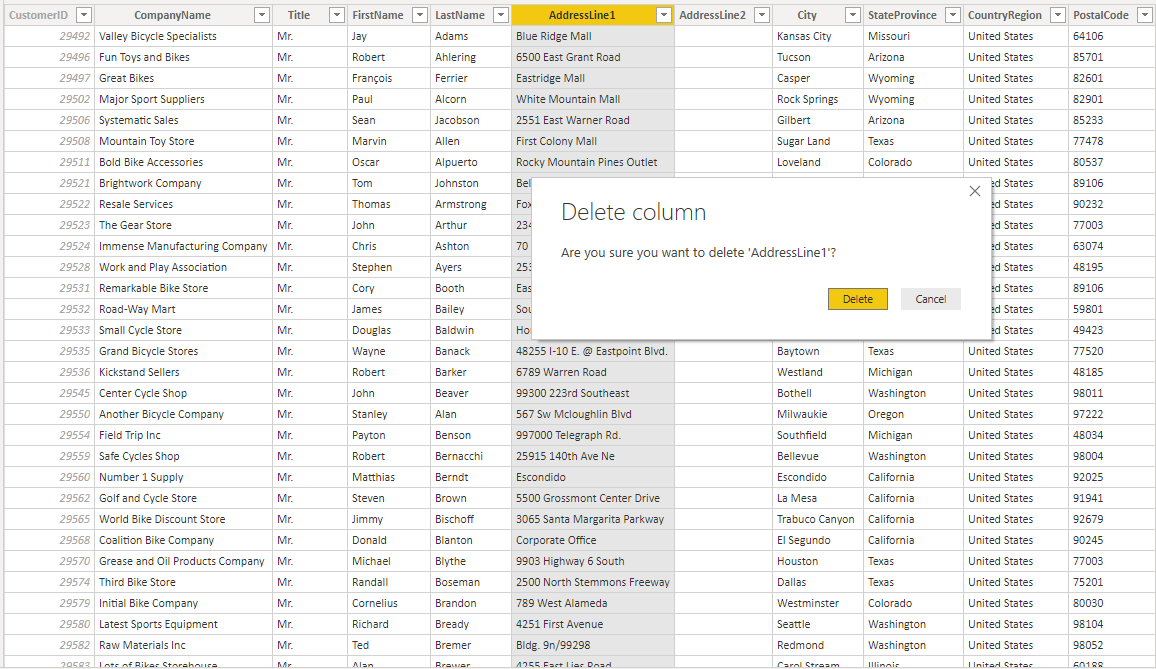
\includegraphics[width=15cm]{images/33}\newline
\end{center}
\begin{center}
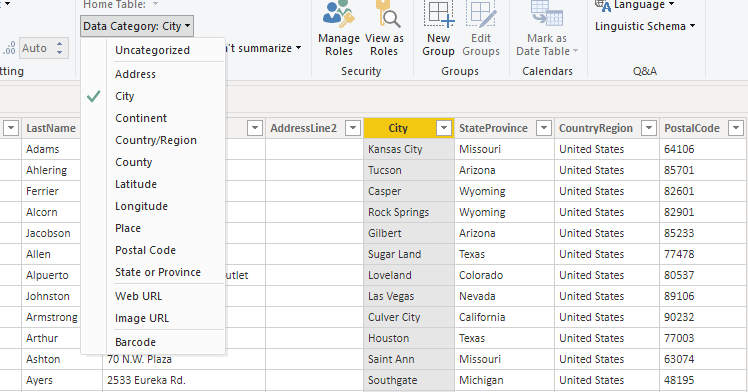
\includegraphics[width=16cm]{images/44}\newline
\end{center}
\begin{center}
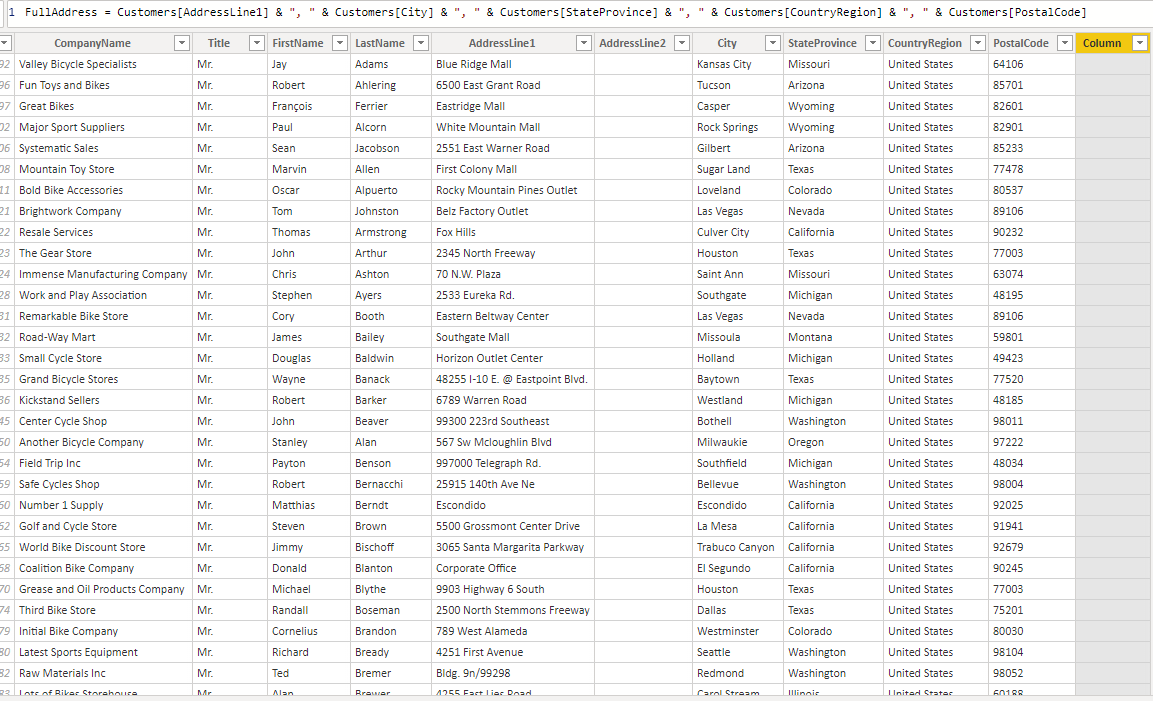
\includegraphics[width=16cm]{images/55}\newline
\end{center}
\begin{center}
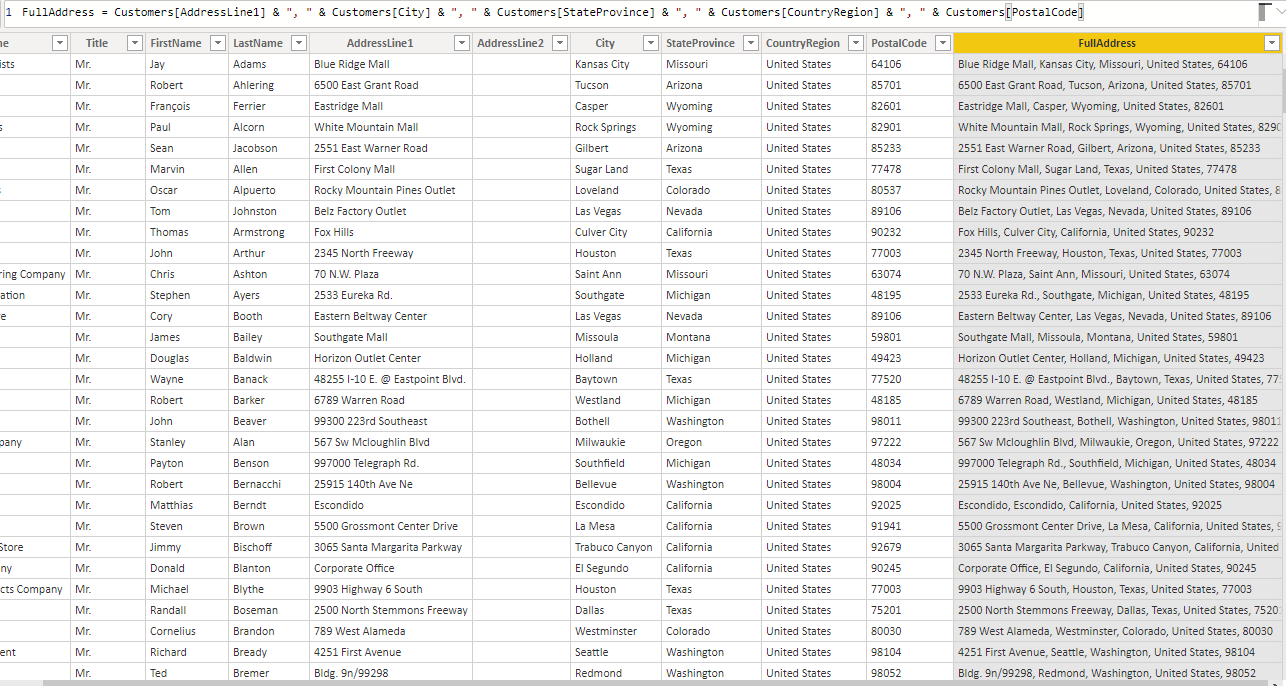
\includegraphics[width=16cm]{images/66}\newline
\end{center}
\begin{center}
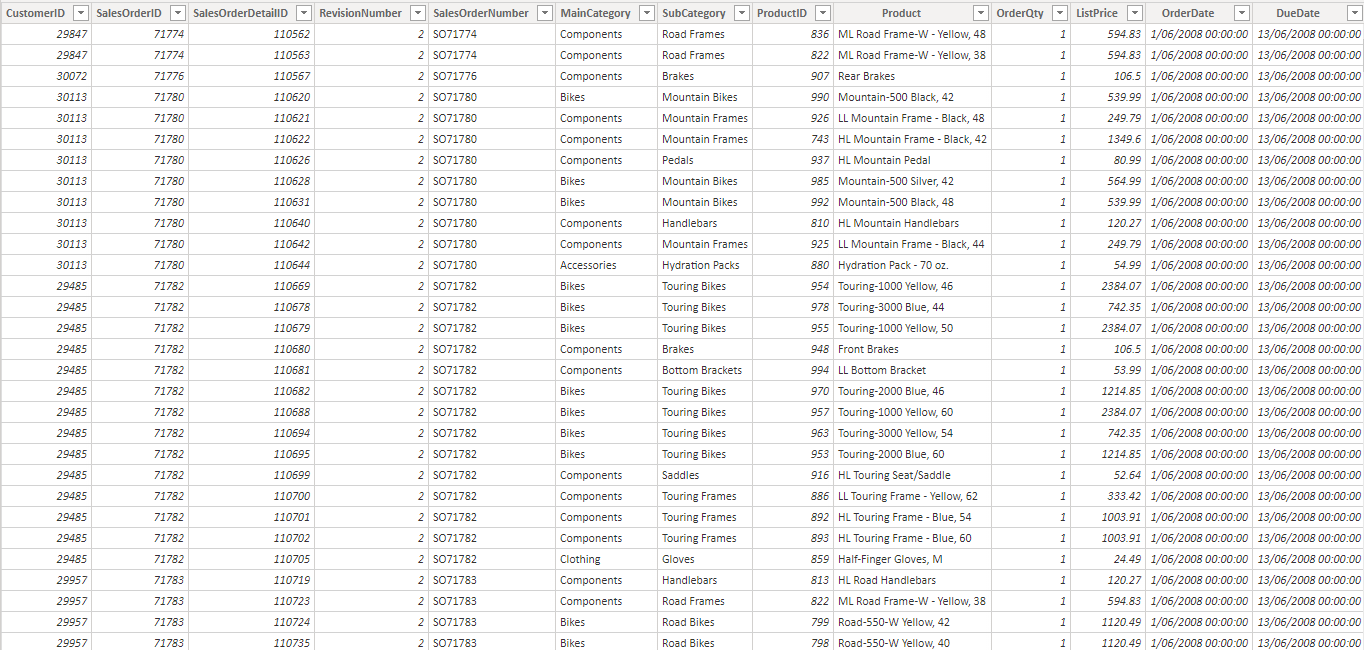
\includegraphics[width=16cm]{images/77}\newline
\end{center}
\begin{center}
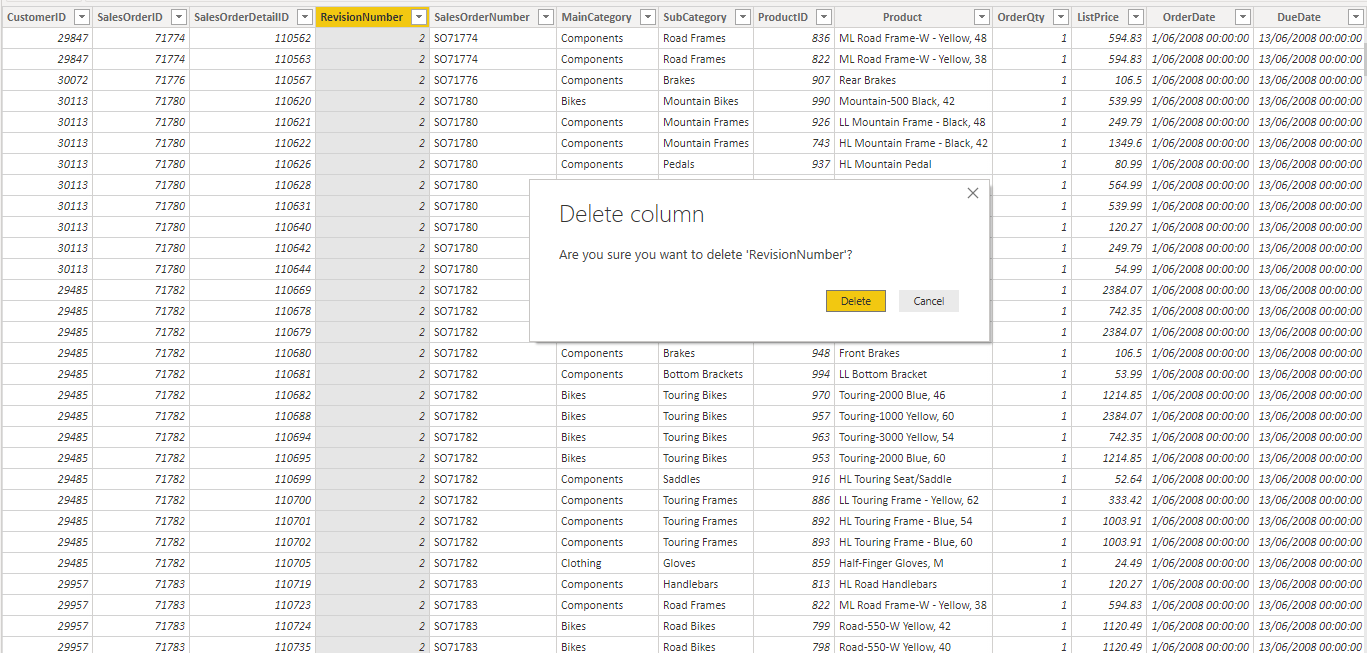
\includegraphics[width=16cm]{images/88}\newline
\end{center}
\begin{center}
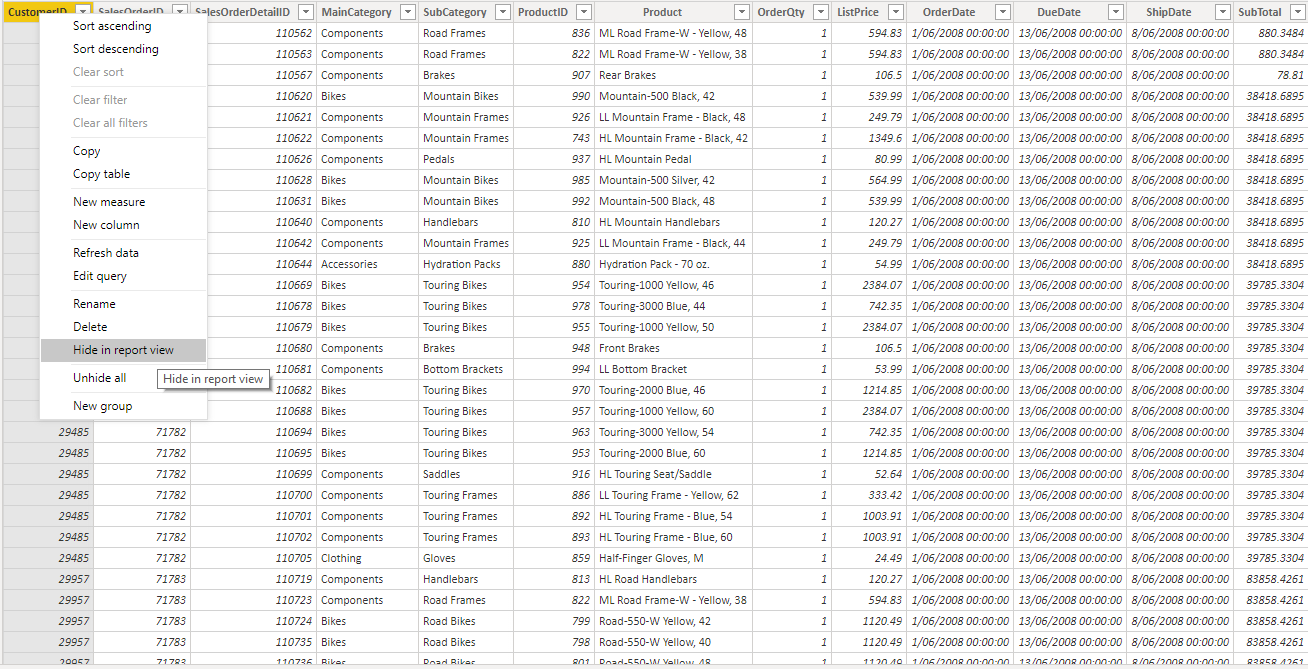
\includegraphics[width=16cm]{images/99}\newline
\end{center}
\begin{center}
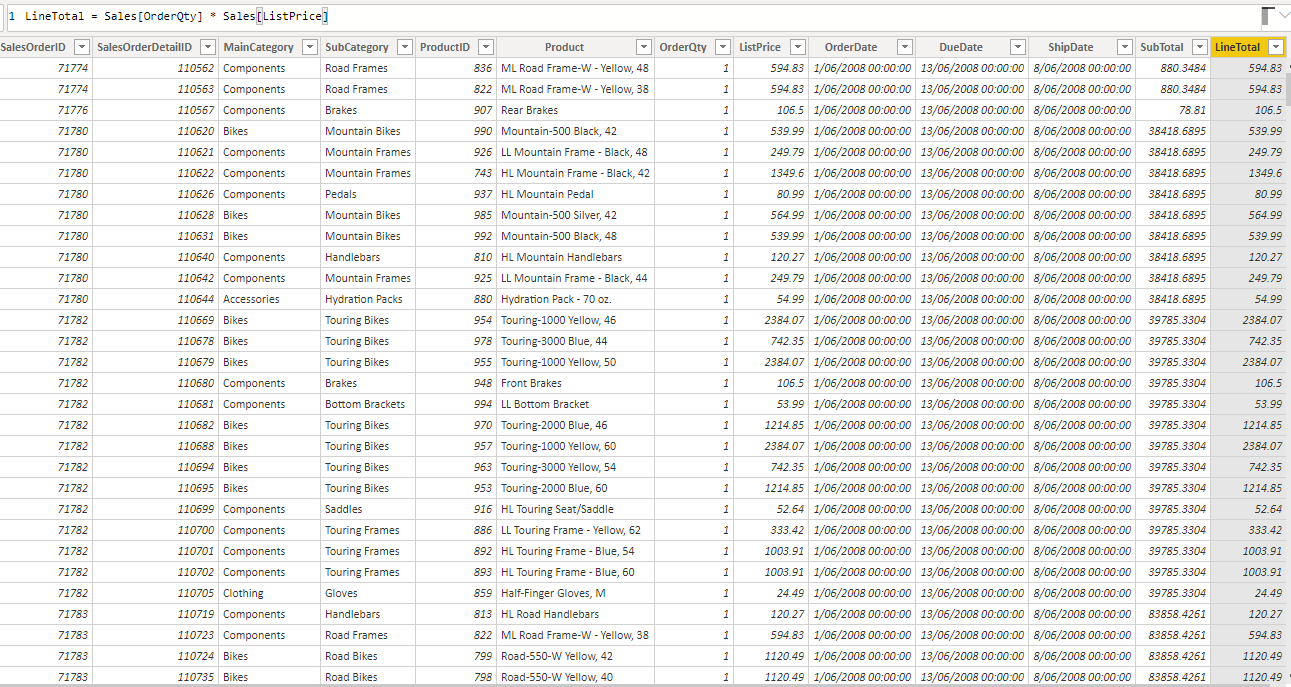
\includegraphics[width=16cm]{images/111}\newline
\end{center}
\begin{center}
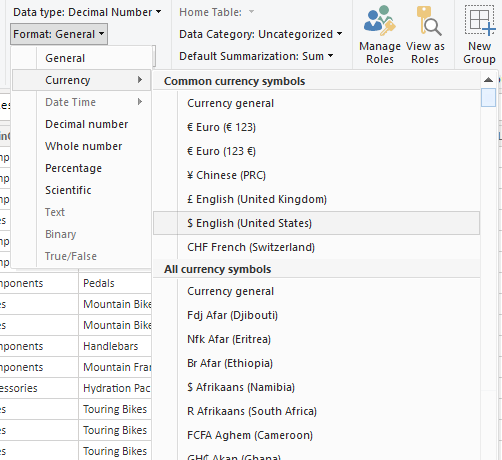
\includegraphics[width=10cm]{images/222}\newline
\end{center}
\begin{center}
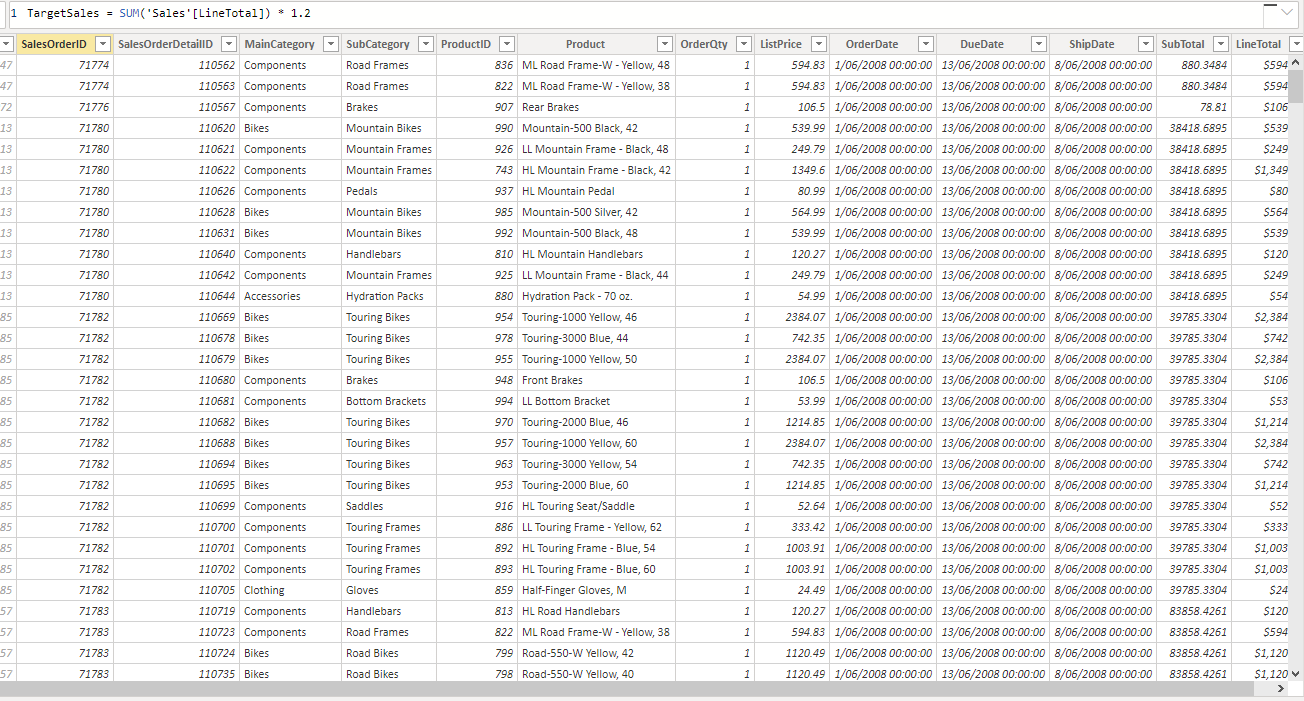
\includegraphics[width=16cm]{images/333}\newline
\end{center}
\subsection{Tarea 3: Combinar Data}
\section{Ejercicio 2: Construyendo Reportes en Power BI} 
\subsection{Tarea 1: Crear un Gráfico}
\subsection{Tarea 2: Crear una Visualización de Mapa}





\end{document}